\section{Computational methods} \label{s:computational}


\acrfull{ml} and \acrfull{ai} have become buzz words in the past 10 years which have largely been due to the breakthroughs in difficult problems like Computer Vision\cite{Krizhevsky2012-qa} coupled with the increase in computational power. There is usually confusion between the ML \& AI terms, the former represents a subfield of the AI \cite{Domingos_Pedro2015-xr}. In the "Master Algorithm", \citet{Domingos_Pedro2015-xr} defines that the goal of the AI field is to make computers learn better than humans. This has been turned in popular culture to have three milestones, turned into three stages of AI: narrow, human-level and general AI. Currently, we don't have anything remotely close to human-level and arguably we are a long way\footnote{See paper "Artificial intelligence hits the barrier of meaning" by \citet{Mitchell2019-hv}}. For example, in Computer Vision, the models can detect complex patterns and score high in classifications problems but the algorithm doesn't create any meaning or complex representation of the object classified. These limitations can be seen in the failed promises from Tesla, Waymo and other companies seeking to achieve full self-driving cars\footnote{Dr F. Piekniewski is an AI researcher who has a more cynical view of the AI progress and the big claims some popular tech figures do. Specifically, on self-driving cars, its blog post is interesting \cite{Piekniewski2021-if}.}.  Similarly, for the Large Language Models (LLMs) like ChatGPT or Bard which massively advanced the chatbots but the models still can not form an understanding of the real world. Thus, one can see the AI term as more of an aspiration to which the field aims.

Machine Learning represents the collection of tools that are used in Artificial Intelligence development. According to \citet{Domingos_Pedro2015-xr}, there are five schools of thought in this area: the Symbolists, Analogizers, Bayesian, Connectionists, and Evolutionary. Symbolists are looking at drawing knowledge from logic symbols while the Analogizers are extrapolating information from mathematics and logic\cite{Domingos_Pedro2015-xr}. Connectionists and Evolutionary approaches take inspiration from biology, the former from the brain and the latter from Darwinian evolution. Bayesians are concerned with the uncertainty and are dealing with that probabilistic inference through Bayes's theorem\cite{Domingos_Pedro2015-xr}. As the readers will see in the following chapters most of the current work in bioinformatics is using Connectionists, Bayesian and sometimes Evolutionary approaches.

From an ML stance, learning can be of three types: supervised, semi-supervised and unsupervised learning. The first case is when the human labels the data, the corollary being that there is a need for careful processing as well as already having information about the data. This is the 'easiest' case as it comes with a wealth of information and the output is known to belong to the pre-defined set of labels. In this are the most recent progress in \acrfull{dl} was made but it's not a realistic scenario as labelling data is usually challenging and expensive. The semi-supervised (or \acrfull{rl}) is when the model is not given labelled data to learn from, but a set of rules from where it needs to find the solution. This approach has met some successes through \acrfull{dqn} which achieved human skills at Atari games\cite{Mnih2015-cw} or AlphaGo Zero\cite{Silver2017-sw} which is the best Go player in the world. 

As the name suggests the unsupervised learning is the case where there is no input from a human. These computational approaches are used when there is not enough data about the problem, what to expect and patterns are hard to define. Clustering is the prevalent algorithm, that is to find patterns in data which then can be validated with domain knowledge. This is the common scenario in biological applications that data is not labelled, unsupervised approaches are used as seen in \cref{s:rnaSeq}.


\textbf{Revise this after structuring}. The Chapter starts by covering the clustering techniques (\ref{s:clustering}) to support the concepts in consensus subtyping (\ref{s:rnaSeq}). Popular dimension reduction algorithms are widely in genomics where there is a high number of features and are covered in section \ref{s:dim_red}. This is followed by EA (\cref{s:ea_overiew}) and Graph Theory (section \cref{s:graph_overview}) basics in order to support some of the work presented in \cref{s:mutations} and \ref{s:lit:multi-view}. Next \acrlong{ann} are introduced covering concepts like Autoencoders or Spiking Neural Networks, the first is needed for \cref{s:autoencoders}. Lastly, the Neuroevolution \cref{s:neuroevolution} introduces concepts on how to combine the evolutionary with the connectionist approach. 

\subsection{Clustering} \label{s:clustering}

Clustering algorithms have many variations and these are best covered in a code sample\cite{Scikit-learn_undated-ax} from the Scikit-learn library\cite{Pedregosa2011-ts}. A selection of the methods which worked on this project are displayed in \cref{fig:clustering_types}. The rows represent different types of datasets and the columns are the algorithms covered in this document: K-means being a general-purpose algorithm, Ward and Agglomerative both being hierarchical clustering, but Agglomerative is peforming pair-wise grouping. It is worth mentioning, that a modified version of the Scikit-learn code was adapted to the project needs, enabling the run pf multiples clustering techniques with varied parameters to the JBU and TCGA datasets. 

\begin{figure}[!htb]
  \centering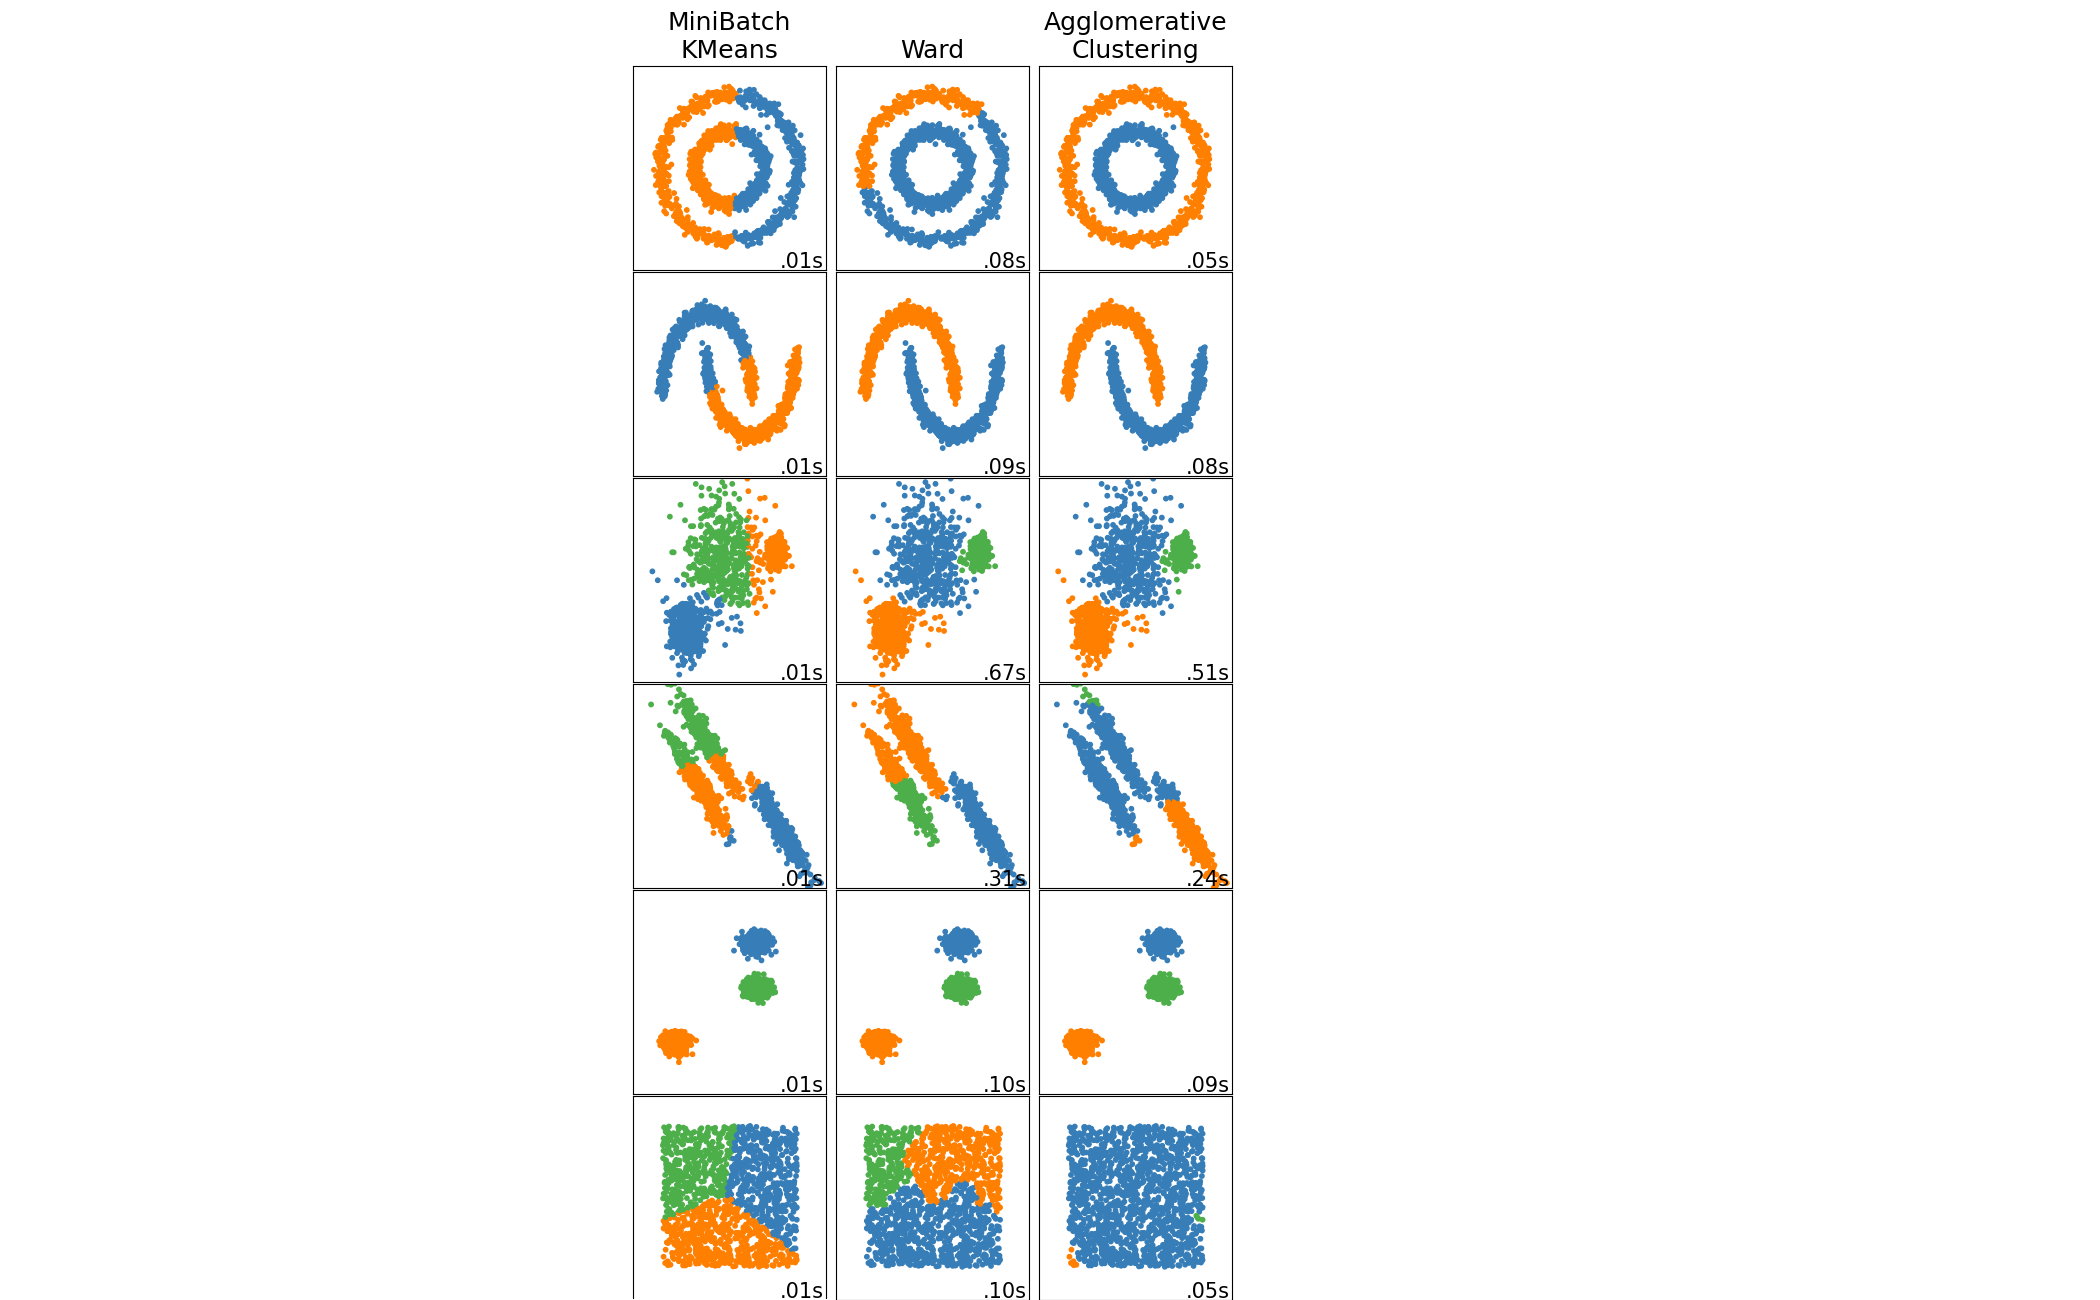
\includegraphics[width=0.8\textwidth,height=0.5\textheight,keepaspectratio]{Images/Clustering/scikit_selected.png}
    \caption{How the algorithms covered in this document behave with different datasets (rows). Image adapted from \cite{Scikit-learn_undated-ax}}
    \label{fig:clustering_types}
\end{figure}
\FloatBarrier

One of the most popular methods (and the simplest) is K-means clustering which tries to find patterns in the data by grouping the data points by distance. There are variations of the algorithms where the datasets are split into multiple batches to improve performances (see \textit{MiniBatch Kmeans} from  \cref{fig:clustering_types}); or Fuzzy K-means that output the cluster membership of each data point. This means, that apart from the cluster labelling there is additional information about how close each point is to a cluster\footnote{For example, if there are 3 clusters, a data point might be 90\% in cluster 1, 6\% in cluster 2 and 4\% in cluster 3.}. From the below K-means pseudocode\footnote{Pseuscode is an accessible method to describe an algorithm.} (\cref{code:k-means}) a few things are worth emphasizing:

\begin{itemize}
  \item The number of centroids (K) is defined by the user.
  \item The distance between two points can be of different types. The euclidean is common, but for higher-dimension cosine is more suitable.
  \item Even though the centroids are randomly initialised new values is computed at each step by averaging the distance of the points in that cluster to the old centroid.
  \item The algorithm converged when the centroids don't significantly change.
\end{itemize}

\begin{lstlisting}[caption={K-means pseudocode}, label={code:k-means}]
  Initialise the centroids at random positions
  while not converged 
    For each data point
      Compute the distance to all the centroids
      The closest represents the cluster to which the data point belongs
    Update the centroids based on the mean distance of each cluster
\end{lstlisting} 

Agglomerative clustering is a type of hierarchical clustering that starts from considering each data point to be its cluster, then, computes higher up groups based on the given linkage method. These algorithms (pseudocode in \cref{code:agg_clustering}) build hierarchical trees and can be seen visually in dendrogram figures (\textbf{like in \cref{fig:dendogram} form Appendix \ref{ap:dendogram}}) which are useful in visualising the clustering evolution. Both K-means and Agglomerative Clustering can use different types of distances, but the latter does not require to set the number of centroids, but the linkage needs to be set. This setting configures the algorithm how the datapoint grouping is performed and the Scikit-learn supports the following\footnote{
  There is a nice visualisation for each of these hierarchical clustering in this \href{https://towardsdatascience.com/machine-learning-algorithms-part-12-hierarchical-agglomerative-clustering-example-in-python-1e18e0075019}{Medium post} }:
\begin{itemize}
  \item Average - Grouping is done by the average distance between cluster points.
  \item Ward - Merging clusters by the sum squared distances. This linkage minimizes the variance and it's similar to K-means.
  \item Single - The distance between two groups is given by the two closest points. Think of this as considering clusters to be merged that have the closest point.
  \item Complete - The opposite to Single linkage, the distance between the two groups is given by the farthest points. In this case, we look at the outer layer points and it may give a more accurate grouping.
\end{itemize}


\begin{lstlisting}[caption={Agglomerative hierarchical clustering pseudocode, style=\small}, label={code:agg_clustering}]
  To each data point assign a cluster number
  while more than one cluster
    Group the closest datapoints together 
    Smaller clusters morph together into a larger ones
\end{lstlisting} 

\subsubsection*{Clustering metrics}

One of the challenges in clustering is to measure the performance of grouping as there is no labelling or prior information on how the grouping should look like. This project uses the canonical metrics which are supported by Scikit-learn\cite{Pedregosa2011-ts,Scikit-learn_undated-ax}. These are:
\begin{itemize}
  \item Silhouette Coefficient - higher the better. A higher Silhouette Coefficient score relates to a model with better-defined clusters. 
  % It can use different distances and the score is calculated per sample as it follows:
  % \begin{itemize}
  %   \item The mean distance between a sample and all other points in a class.
  %   \item The mean distance between a sample and all other points in the next nearest cluster.
  %   \item The total score for the dataset is the mean of the above two points.
  % \end{itemize}
  \item Calinski-Harabasz Index - higher the better. A higher Calinski-Harabasz score relates to a model with better-defined clusters.  The score is the index is the ratio of the sum of between-clusters dispersion and of inter-cluster dispersion for all clusters (where dispersion is defined as the sum of distances squared).
  \item Davies-Bouldin Index - lower the better. A lower Davies-Bouldin index relates to a model with better separation between the clusters. The index is the average ‘similarity’ between clusters, where the similarity is a measure that compares the distance between clusters with the size of the clusters themselves.
\end{itemize}


In addition to the above metrics, there is a popular heuristic procedure, the Elbow method, which aids in choosing the right number of clusters. In \cref{fig:elbow_method} the y-axis is represented by the distance of the points from their centroids, while the x-axis is the number of clusters. It can be seen that there is a point of inflexion when the number of clusters is set to five and that is considered to be the optimal number of clusters.

\begin{figure}[!htb]
  \centering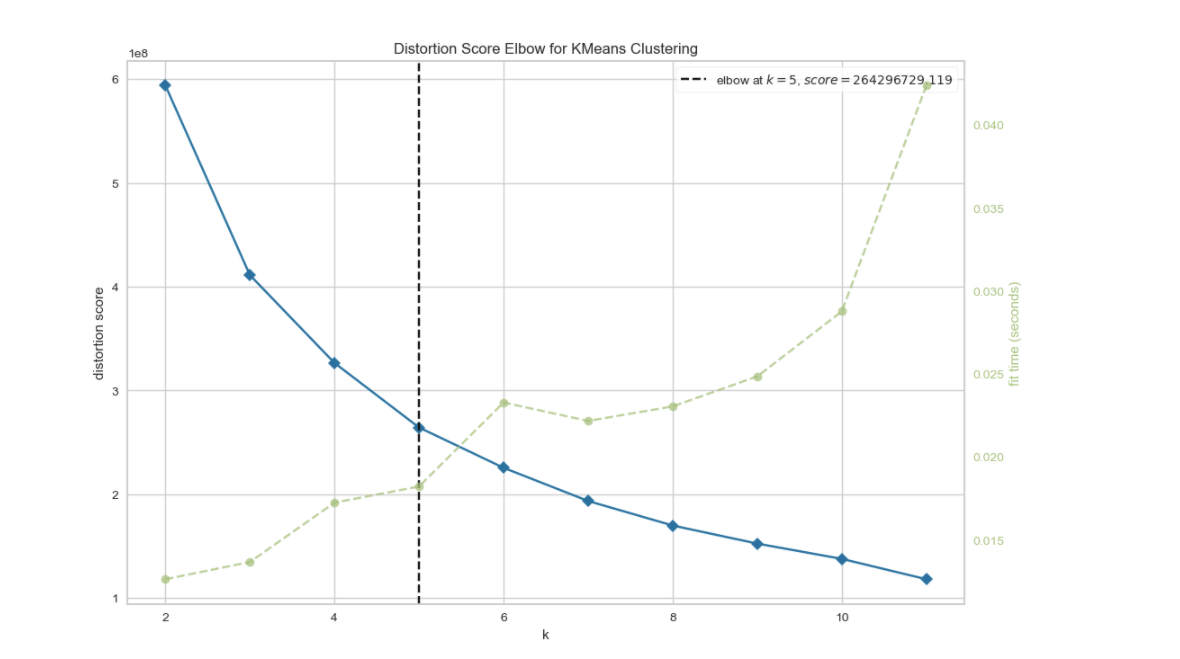
\includegraphics[width=0.9\textwidth,height=0.5\textheight,keepaspectratio]{Images/Clustering/elbow_method.png}
    \caption{Example of the elbow method, where 5 clusters are the optimal number of clusters. This has been applied on unplubished data of Bening Uropathies from Jack Birch Unit. The green line is the computational time. }
    \label{fig:elbow_method}
\end{figure}
\FloatBarrier


\subsection{Dimension reduction} \label{s:dim_red}

In contrast to many computationally- or physics-focused data analysis problems, biologically derived datasets are characterised by a high number of features (dimension) and a small number of samples. Thus, it is often essential to use dimension reduction, \acrfull{pca} is the standard method that works by projecting the higher dimension to the specified lower dimension. For example, a principal component of a genomic dataset might be linked to biological sex, as it influences many features of a biological system.

However, this doesn't accommodate well with non-linear patterns for which \acrfull{umap} and \acrfull{tsne} are used. Both are stochastic and non-linear dimension reduction techniques widely used in bioinformatics. UMAP is gaining popularity as it's been more stable in representing both within and between cluster sample relatedness.

Another dimension reduction technique is \acrfull{nmf} which operates on the same principles as PCA which is by finding a matrix of a lower rank with the minimum information loss. This means that the features present in the data are preserved better when reduced to lower dimensions while the ones that do not contribute to the data resolution are discarded. In addition, NMF conserves the non-linear aspects of the data and a Bayesian version was used in the \acrfull{tcga} classification by \citet{Robertson2017-mg}. NMF also were used in the works of propagating (mutation) data into the networks by \citet{Yang2016-dm, Cai2008-fv} and covered in \cref{s:lit:net_prop}.



\subsection{Evolutionary Algorithms} \label{s:ea_overiew}

% In the previous section described how graphs are used to analyse the gene interactions and a similar approach but the different algorithm is \acrfull{cgp}. This is part of the \acrfull{ea} family which draws inspiration from the Darwinian evolution.

\acrlong{ea} are a type of \acrshort{ml} that draws inspiration from Darwinian evolution. By incorporating random changes in the algorithm, EA can be used for optimisation or search problems. Thus, EAs are suitable for doing a wide search of the solution space\footnote{Imagine the solution space as space of the total possible solutions for a problem.} which means that they might find an unusual solution and escape the local minimum. A useful analogy here is to think as one climbing a mountain (search space), the goal (optimal solution) is to reach the highest peak but along the way, there are other peaks (local minimum) but smaller (less optimal) than the highest peak (optimal solution). The process (algorithm) in reaching the desired peak is incremental and it requires choosing the right path to reach the global top. Usually, an algorithm has difficulties in differentiated between the highest peaks and the smaller ones, but due to the high variation characteristic of EA, these methods perform well in such problems.


However, these algorithms have a high computational cost and do not usually scale well, therefore are applied to relatively small problems (i.e. number of features). The corollary is that EAs are easier to understand compared to the  \acrfull{dl} (explored in \cref{s:dl_genomics}) and are classified as a 'white-box' approach. In \cref{s:mutations} is presented the MDPFinder (\citet{Zhao2012-wj}) model where \acrfull{ga}, a simpler version of EAs, are applied to process both Gene Expression and mutations.

% would split the sentence here. You could then link to your next point, perhaps: "...from Darwinian evolution. By incorporating random changes in the parameters of a model, or set of models, EA can be used for optimisation..." Something like this makes it clearer why the Darwinian principles are important

As EA resembles the evolutionary process there is also some shared terminology, an individual in the EA context represents a potential solution and a population is a collection of potential solutions. \Cref{fig:ea_basic} describes the algorithmic flow of the evolutionary approach which starts with the initialisation stage, where the individuals are given (usually) random values, followed by the second stage where the fitness of the individuals is measured; i.e. how suitable they are for the problem. If the problem is not solved, then select only the fittest individuals which are then mutated/crossover, introducing variation to the new population. Like in biology, this last step, gives EA a large variety of individuals. This set of steps is run until an individual fits the solution/problem. It is worth mentioning, that the mutation rate, crossover and how the individual is selected, are preset parameters. 

\begin{figure}[!htb]
  \centering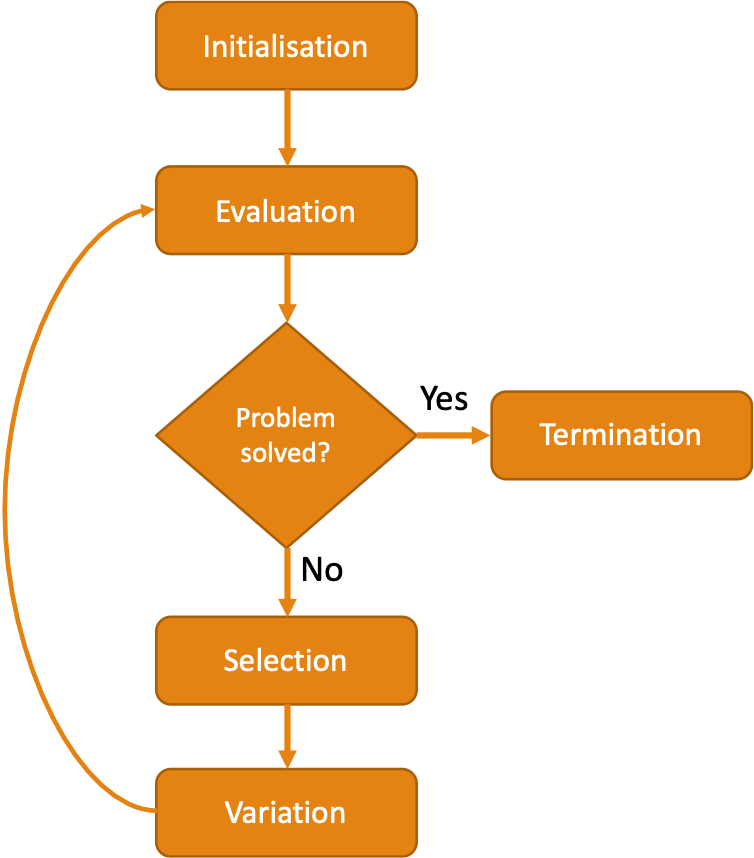
\includegraphics[width=0.4\textwidth,height=0.4\textheight,keepaspectratio]{Images/Resources/EA_basic.png}
    \caption{Evolutionary Algorithms algorithm.}
    \label{fig:ea_basic}
\end{figure}
\FloatBarrier


Defining the fitness function as well as encoding the data for the EA algorithm is one of the challenges when developing EA as it is problem specific. Biological evolution is a process that takes time and many iterations, the in-silico adaptation share that and it is the reason for not scaling well or as it has a high computational cost.

The MDPFinder model presented in \cref{s:mutations} used a variation of EA, called \acrfull{ga} which is a simpler version of the EA family where individuals resemble the chromosome. \acrfull{cgp} is another EA algorithm which it's used to process graph representation and it overcomes some of the limitations of the simpler EA methods. As we've seen that graph representation it's already been used in gene networks, CGP may represent an interesting venue to follow. 


\subsection{Artificial Neural Networks} \label{s:ann_overview}

As it was mentioned at the beginning of this chapter, the connectionist approach is what drives the current AI hype and it's due to the advances in both algorithms and computational power. The inspiration comes from how the brain draws the information from the external stimuli, stores it in memory and retrieve it. Despite being many unknowns to the brain, the main components that are involved in the learning process are the neurons and the synapses between them\footnote{The neurons and synapses are the main components, but there may be others like dendrites which can also be computational units as seen later in the section.}. The simplest learning rule was introduced by Donald Hebb which states "Neurons that fire together, wire together"\cite{Hebb_Donald1949-nn}. This means that a neuron that fire or its concurrently activated with another one (or in a given time window) the two form a stronger connection. The opposite is true, the synapse is weaken, when two neurons that do not get activated in the same time window.

\Cref{fig:ann_basic} it's a simple, single-layer, feed-forward Neural Network where a layer represents a collection of units that usually have the same activation function. In the case of \acrfull{dnn}, the ANN is constructed by many such layers with a large number of units. The neurons are the computational component, each having an activation function that 'tells' the unit when to activate and send a signal across the synapse. The connections between the units are assigned a weight that gives the strength of the synapses. The information is stored in the connections between the units, and it follows Donald Hebb's learning rule stated earlier. Therefore, the central goal of ANN is to find the specific combination of weight values that gives the desired output. Previously, we mentioned different types of learning, in the supervised case, there is an algorithm that has been the engine of the connectionist approach, called back-propagation. As the name suggests, this method propagates the input's error from the output layer back, this information is used then to compute new values for the network's weights; this is called stochastic gradient descent.
%  This algorithm is not used in the biological NN and it relies on the data given and may inherit its biasis\footnote{For example the data is collected only for a specific demographic.}. 

\begin{figure}[!htb]
  \centering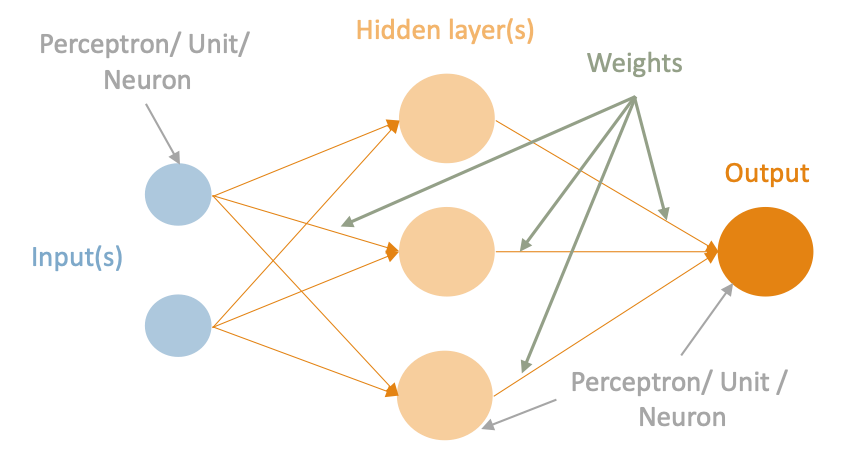
\includegraphics[width=0.7\textwidth,height=0.7\textheight,keepaspectratio]{Images/ANN/Basic_ANN.png}
    \caption{A Simple ANN architecture. }
    \label{fig:ann_basic}
\end{figure}
\FloatBarrier


\paragraph*{Autoencoders} \label{s:autoencod_overview}

Autoencoders are a particular type of Deep Neural Networks and \cref{fig:autoencoders} represents a diagram a simple Autoencoder architecture in which it can be seen that there are 3 main components. The input layer to which the data is fed, for more complex models it has additional hidden layers and with the input, the two layers are known together as the encoder stage. The bottleneck part is where the data is compressed into a lower dimension. Next, a mirror to the encoder, the decoder, is dealing with reconstructing the outputs of the bottleneck into original data; hence, the name. This part of autoencoders is an advantage over the PCA as the original data can be reconstructed from the lower dimension. A derivative of Neural Networks, autoencoders are more suitable to find non-linear patterns in the data as whereas PCA finds only linear patterns. With all these advantages as dimension reduction techniques is not a surprise that there has been some work on applying Autoencoders to genomics (explored further in \cref{s:autoencoders}).

\begin{figure}[!htb]
  \centering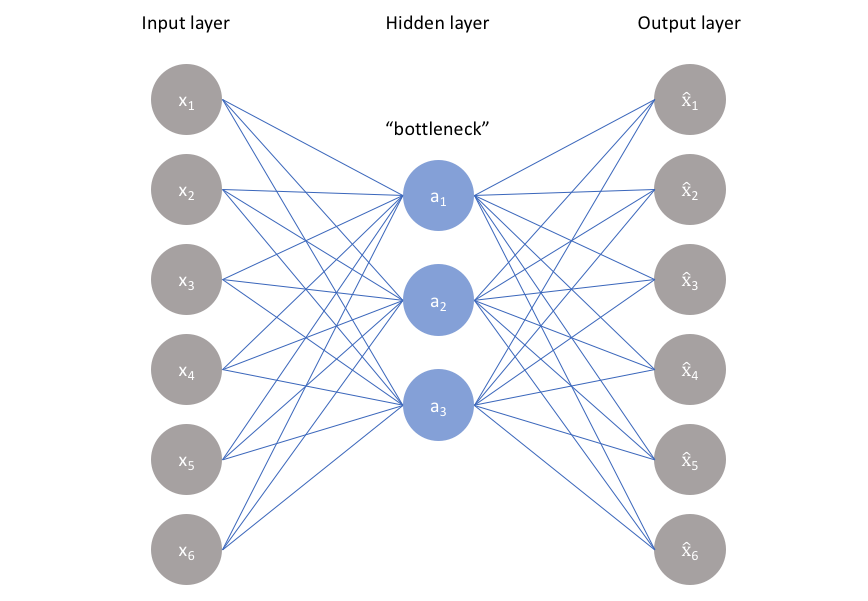
\includegraphics[width=0.8\textwidth,height=0.5\textheight,keepaspectratio]{Images/Autoencoders/simple_autoencoders.png}
    \caption{Simple architecture of autoencoders, from \cite{Jordan2018-bc}}
    \label{fig:autoencoders}
\end{figure}
\FloatBarrier

Autoencoders are the most successful \acrshort{dnn} approaches to genomics problems where they have been used as a dimension reduction technique to solve the dimension curse of genetic data, where few samples are available with a large number of features (genes). This means, that they are not replacing the clustering models but techniques like \acrfull{pca} or \acrfull{nmf}, and will be used in conjunction with clustering techniques.



\subsection{Graph Theory} \label{s:graph_overview}

One of the aims of graph theory is to find the influence nodes, which in biology this might be the case of finding the driver genes which are the ones with the biggest impact on the network. In \cref{fig:graphs_basic} it's a simple representation of a graph, where a node (or vertices) is a gene and the edge between them is the connection. 

To establish how genes are linked to a network and interact,  the edges are assigned values that enforce the link between nodes (genes) and this data can be put into a table that can be processed by different graph algorithms. As one of the goals of this project is to understand how genes interact and their network effect, \cref{s:lit:multi-view} covers how graph theory is applied in multi-omics. Apart from being able to find the driver genes graphs are a good tool to visualise the gene interactions. 

\begin{figure}[!htb]
  \centering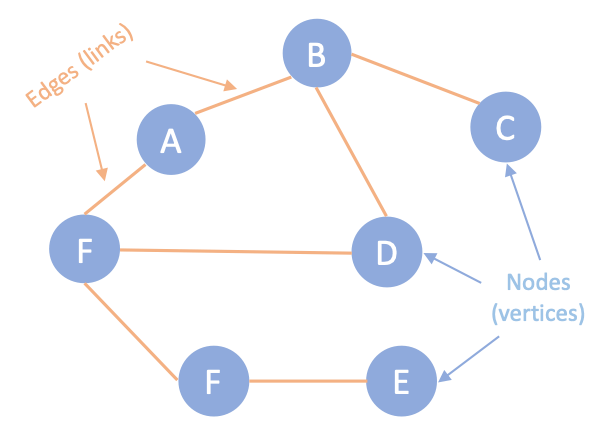
\includegraphics[width=0.5\textwidth,height=0.5\textheight,keepaspectratio]{Sections/Lit_review/Resources/basic_graphs.png}
    \caption{Basic graphs.}
    \label{fig:graphs_basic}
\end{figure}
\FloatBarrier


% Keep this section simple. It links to parts of your project you haven't discussed yet and so becomes a bit unclear. Effectively you want to state that genes can be linked in a network and that many biological approaches allow measurements of genes. This means you can infer relationships, see how relationships change in disease/perturbation and assess how distinct, but linked-in-the-network perturbations can lead to a common result/phenotype/observation


\subsection{Choosing the right ML approach} \label{s:neuroevolution}

\Cref{s:ea_overiew} covered the basics of the evolutionary approach, and in both \ref{s:ann_overview} \& \ref{s:autoencod_overview} sections it was presented the connectionists' view of ML. These two solve different types of problems, where so far, the EAs are better for search problems and the ANNs for classification. The ANNs work by finding an optimal configuration of the weights and network topology, which can be seen as a search/optimisation problem for the right network configuration. Therefore, there has been work in combining the two approaches in what is called Neuroevolution. Such an approach has been used to process mutations data and it's covered in \cref{s:mutations}.

In these computational methods, EAs are used to find the optimal initial configuration of the ANN, which then it's used to be trained. Starting from a different than random state helps the ANN to avoid the local minimum problem, and to increase the classifications performances. On top of that, the EAs are also used to determine the best network topology which means the number of layers, units, their connections, etc.

Therefore, choosing the right ML depends on the problem statement as EA and ANN are good in specific situations, but can also be combined to take advantage of both worlds. The next section attempts to cover the work done across the genomics field by looking at various approaches depending on the datasets used.


% s is a nice section summary style paragraph - "look there are these methods with different strengths, so need to choose carefully, but sometimes we can combine". I would maybe rename this "Choosing the correct ML approach" (or similar) and use it to round off the whole section and link into the next


% \import{./}{general_ml.tex}

% \import{./}{ea.tex}

% \import{./}{snn.tex}